\documentclass[aspectratio=169]{beamer}
\usepackage{tikz}
\usepackage{newpxmath, newpxtext}
\usefonttheme[]{serif}

\title{Numerical Calculation of 1-d Dimensional Heat Equation}
\author{Taro Morita}

\begin{document}
\begin{frame}
    \titlepage
\end{frame}

\begin{frame}
    \frametitle{Heat Equation}
    \framesubtitle{Explicit method}
    \begin{equation}
        \frac{\partial \theta}{\partial t} = \kappa \frac{\partial^2 \theta}{\partial x^2}
    \end{equation}
    Recurrence formula is ...
    \begin{equation}
        \frac{\theta_{i, j+1} - \theta_{i, j}}{\Delta t} = \kappa \frac{\theta_{i-1, j} - 2 \theta_{i, j} + \theta_{i+1, j}}{(\Delta x)^2}
        \label{eq:2}
    \end{equation}
\end{frame}

\begin{frame}
    \frametitle{Heat equation}
    \framesubtitle{Explicit method}
    Transforming equation \ref{eq:2}, we get
    \begin{equation}
        \theta_{i, J+i} = r \theta_{i-1, j} + (1 - 2 r) \theta_{i, j} + r \theta_{i-1, j}
    \end{equation}
    Where $r = \kappa \displaystyle{\frac{\Delta t}{(\Delta x)^2}}$
\end{frame}

\begin{frame}
    \frametitle{Heat equation}
    \framesubtitle{Explicit method}
    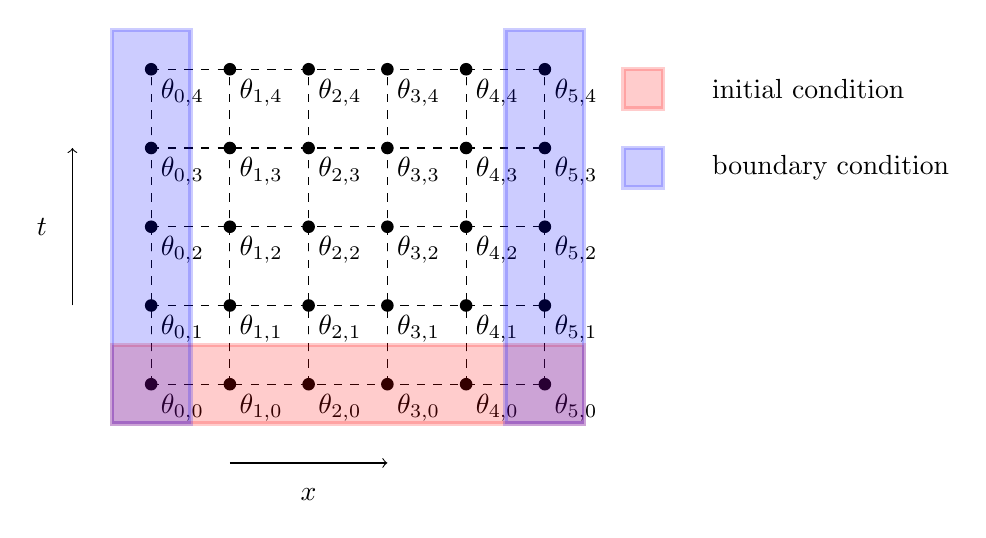
\begin{tikzpicture}
        \centering

        \foreach \y in {0, 1, ..., 4}
        {
            \draw [dashed] (0,\y) -- (5,\y);
            \foreach \x in {0, 1, ..., 5} 
            {
                \draw [dashed] (\x,0) -- (\x,4);
                \fill (\x,\y) circle [radius=0.08];
                \coordinate [label=below right:$\theta_{\x, \y}$] (0) at (\x, \y);
            }

        }
        \draw[->] (1,-1) -- (3, -1);
        \draw[->] (-1, 1) -- (-1, 3);
        \coordinate [label=below : $x$] (x) at (2, -1.2);
        \coordinate [label=left : $t$] (t) at (-1.2, 2);
        \draw [ultra thick, draw=red, fill=red, opacity=0.2] (-0.5, -0.5) -- (5.5, -0.5) -- (5.5, 0.5) -- (-0.5, 0.5)--cycle;
        \draw [ultra thick, draw=blue, fill=blue, opacity=0.2] (-0.5, -0.5) -- (0.5, -0.5) -- (0.5, 4.5) -- (-0.5, 4.5)--cycle;
        \draw [ultra thick, draw=blue, fill=blue, opacity=0.2] (4.5, -0.5) -- (5.5, -0.5) -- (5.5, 4.5) -- (4.5, 4.5)--cycle;
        \draw [ultra thick, draw=red, fill=red, opacity=0.2] (6, 3.5) -- (6.5, 3.5) -- (6.5, 4) -- (6, 4)--cycle;
        \draw [ultra thick, draw=blue, fill=blue, opacity=0.2] (6, 2.5) -- (6.5, 2.5) -- (6.5, 3) -- (6, 3)--cycle;
        \coordinate [label=right: initial condition] (I) at (7,3.75);
        \coordinate [label=right: boundary condition] (I) at (7,2.75);
    \end{tikzpicture}
\end{frame}
\end{document}
